\documentclass[a4paper,12pt]{article}
\usepackage[utf8]{inputenc}
\usepackage[T1]{fontenc}
\usepackage{amsmath, amssymb}
\usepackage{geometry}
\geometry{margin=2.5cm}
\usepackage{graphicx}
\usepackage{wrapfig}
\usepackage{amsfonts}
\usepackage{tikz}

\title{Nombres complexes et Géométrie}

\begin{document}

    \maketitle

    \section*{Dans le programme de :}
    \textbf{Terminale Maths Expertes et Terminales STI2D}

    \subsection*{Prérequis :}
    Construction de l’ensemble $\mathbb{C}$ des nombres complexes, forme algébrique (opérations, propriétés, conjugué), forme trigonométrique (module, argument), suites numériques, transformations géométriques, trigonométrie.

    \section*{Représentation des nombres complexes}
    \section{Forme algébrique}
    \textbf{Propriété :} Tout élément de $\mathbb{C}$ s’écrit de manière unique sous la forme $a + ib$ avec $a, b \in \mathbb{R}$.

    \begin{itemize}
        \item $a$ est appelé \textbf{partie réelle} de $z$, on note $a = \operatorname{Re}(z)$.
        \item $b$ est appelé \textbf{partie imaginaire} de $z$, on note $b = \operatorname{Im}(z)$.
    \end{itemize}

    \textbf{Remarque :}
    \begin{itemize}
        \item Si $a = 0$, on dit alors que $z$ est \textbf{imaginaire pur}.
        \item Si $b = 0$, alors $z = a \in \mathbb{R}$, $z$ est un \textbf{nombre réel}.
    \end{itemize}

    \subsection{Exemples :}

    \begin{itemize}
        \item Soit $z_1$ le nombre complexe tel que $z_1 = 5 - 4i$.
        \begin{itemize}
            \item La partie réelle de $z_1$: $\operatorname{Re}(z_1) = 5$.
            \item La partie imaginaire de $z_1$: $\operatorname{Im}(z_1) = -4$.
        \end{itemize}

        \item Soit $z_2$ le nombre complexe tel que $z_2 = 3,79i$.
        \begin{itemize}
            \item La partie réelle de $z_2$: $\operatorname{Re}(z_2) = 0$.
            \item La partie imaginaire de $z_2$: $\operatorname{Im}(z_2) = 3,79$.
            \item $z_2$ est \textbf{imaginaire pur}.
        \end{itemize}
    \end{itemize}

    \subsection{Définition :}
    Soit $z$ un nombre complexe tel que $z = a + ib$, avec $a$ et $b$ deux nombres réels. Alors, le \textbf{conjugué} de $z$, noté $\overline{z}$, est le nombre complexe défini par
    \[
        \overline{z} = a - ib.
    \]

    \subsection{Exemple :}

    Soit $z$ le nombre complexe tel que $z = 3 - 7i$.

    \begin{itemize}
        \item Le conjugué de $z$ est $\overline{z} = 3 + 7i$.
    \end{itemize}

    \section{Forme trigonométrique}
    \begin{figure}[h]
        \centering
        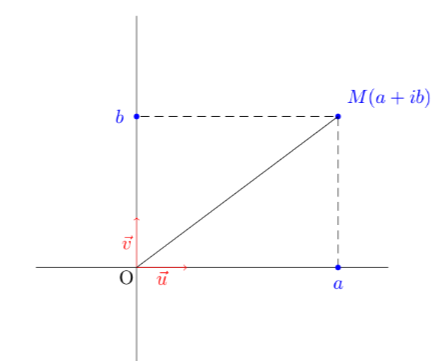
\includegraphics[width=0.3\textwidth]{formealgebrique.png}
        \label{fig:formealgebrique}
    \end{figure}
    \subsection{Définition :}
    Soit $z$ un nombre complexe non nul et $M$ le point d’affixe $z$ (voir figure). On appelle \textbf{argument} de $z$ toute mesure en radians de l’angle $\widehat{(\vec{u}, \vec{OM})}$, avec $\vec{u}$ le vecteur unitaire de l’axe des réels positifs.

    On le note $\arg(z)$. L’argument est défini \textbf{à $2k\pi$ près} ($k \in \mathbb{Z}$).

    \subsection{Remarques :}
    \begin{enumerate}
        \item Si $z$ est un réel, c’est-à-dire $z = a$ :
        \begin{itemize}
            \item si $a > 0$, alors $|z| = a$ et $\arg(z) = 0$.
            \item si $a < 0$, alors $|z| = -a$ et $\arg(z) = \pi$.
        \end{itemize}
        \item Si $z$ est un imaginaire pur, c’est-à-dire $z = ib$ :
        \begin{itemize}
            \item si $b > 0$, alors $|z| = b$ et $\arg(z) = \frac{\pi}{2}$.
            \item si $b < 0$, alors $|z| = -b$ et $\arg(z) = -\frac{\pi}{2}$.
        \end{itemize}
    \end{enumerate}

    \subsection{Propriété : Module et argument de l’opposé et du conjugué}

    \begin{figure}[h]
        \centering
        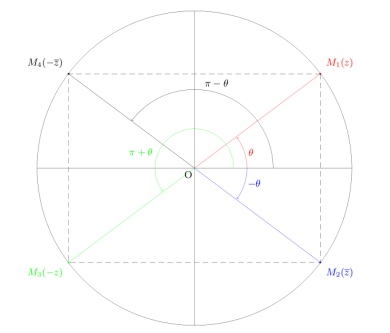
\includegraphics[width=0.6\textwidth]{figure_exemple_trigo.png}
        \caption{Module et argument de l’opposé et du conjugué}
        \label{fig:figure_exemple_trigo}
    \end{figure}

    Soit $z$ un complexe non nul et $M_1$, $M_2$, $M_3$, et $M_4$ les points d’affixes respectives $z$, $\overline{z}$, $-z$ et $-\overline{z}$.

    Comme on peut le remarquer sur la figure \ref{fig:figure_exemple_trigo}, on a les propriétés suivantes :

    \[
        |z| = |\overline{z}| = |{-z}| = |{-\overline{z}}|
    \]

    \[
        \arg(\overline{z}) = -\arg(z) \; [2\pi]
    \]

    \[
        \arg(-z) = \pi + \arg(z) \; [2\pi]
    \]

    \[
        \arg(-\overline{z}) = \pi - \arg(z) \; [2\pi]
    \]

    \section{Forme exponentielle}

    \subsection{Théorème : Fonction exponentielle complexe}

    Soit $f$ la fonction définie sur $\mathbb{R}$ par $f(\theta) = \cos(\theta) + i\sin(\theta)$.

    \begin{itemize}
        \item En utilisant les formules d’addition du cosinus et du sinus, on montre que, pour tous réels $\theta$ et $\theta'$ :
        \[
            f(\theta + \theta') = f(\theta) \times f(\theta').
        \] \\
        En effet, on a : \\
        \begin{align*}
            f(\theta + \theta') &= \cos(\theta + \theta') + i\sin(\theta + \theta') \\
            &= \cos(\theta)\cos(\theta') - \sin(\theta)\sin(\theta') + i(\cos(\theta)\sin(\theta') + \sin(\theta)\cos(\theta')) \\
            &= (\cos(\theta) + i\sin(\theta))(\cos(\theta') + i\sin(\theta')) \\
            &= f(\theta) \times f(\theta').
        \end{align*}
        De plus, $f(0) = 1$.
        \item Par analogie avec la fonction exponentielle dans $\mathbb{R}$, on pose $f(\theta) = e^{i\theta}$, soit :
        \[
            e^{i\theta} = \cos(\theta) + i\sin(\theta).
        \]
        \item On a :
        \[
            |e^{i\theta}| = 1 \quad \text{et} \quad \arg(e^{i\theta}) = \theta \; [2\pi].
        \]
    \end{itemize}

    \subsection{Exemple}

    \[
        e^{i\frac{\pi}{2}} = \cos\left(\frac{\pi}{2}\right) + i\sin\left(\frac{\pi}{2}\right) = i.
    \]

    \subsection{Définition : Forme exponentielle d’un nombre complexe}

    Tout nombre complexe $z$ non nul s’écrit sous la forme :
    \[
        z = r e^{i\theta} \quad \text{avec} \quad r = |z| \quad \text{et} \quad \theta = \arg(z) \; [2\pi].
    \]
    Cette écriture est appelée \textbf{forme exponentielle} de $z$.

    Réciproquement, si $z$ est un nombre complexe tel que $z = r e^{i\theta}$ avec $r > 0$, alors $r = |z|$ et $\theta = \arg(z) \; [2\pi]$.

    \subsection{Exemple}

    Soit $z = 1 + i$. On a :
    \[
        |z| = \sqrt{2} \quad \text{et} \quad \arg(z) = \frac{\pi}{4} \; [2\pi].
    \]
    Donc, la forme exponentielle de $z$ est :
    \[
        z = \sqrt{2} e^{i\frac{\pi}{4}}.
    \]

    \section*{Caractérisations d'ensembles de points}
    \section{Cercles, distance à un point}
    \begin{itemize}
        \item Déterminer l'ensemble des points z complexes tels que $|z - 4| = 5$.
    \end{itemize}
    C'est l'ensemble des points z tels que la distance de z à 4 est égale à 5.
    C'est donc le cercle de centre 4 et de rayon 5.

    %Illustration du cercle
    \begin{center}
        \begin{tikzpicture}
            % Axes
            \draw[->] (-2,0) -- (10,0) node[right] {$\Re(z)$};
            \draw[->] (0,-6) -- (0,6) node[above] {$\Im(z)$};

            % Cercle de centre (4,0) et rayon 5
            \draw[blue] (4,0) circle (5);

            % Centre du cercle
            \fill[red] (4,0) circle (0.1);
            \node[anchor=north] at (4,0) {\textcolor{red}{$4$}};
            \fill[green] (9,0) circle (0.1);
            \node[anchor=north] at (9,0) {\textcolor{green}{$9$}};
            \fill[green] (-1,0) circle (0.1);
            \node[anchor=north] at (-1,0) {\textcolor{green}{$-1$}};
            \fill[green] (4,5) circle (0.1);
            \node[anchor=north] at (4,5) {\textcolor{green}{$4 + 5i$}};
            \fill[green] (4,-5) circle (0.1);
            \node[anchor=north] at (4,-5) {\textcolor{green}{$4 - 5i$}};
        \end{tikzpicture}
    \end{center}

    \section{Médiatrices}
    \begin{itemize}
        \item Déterminer l'ensemble des points z complexes tels que $|z - 2| = |z - 2i|$.
    \end{itemize}
    C'est l'ensemble des points z tels que la distance de z à 2 est égale à la distance de z à $2i$.
    C'est donc la médiatrice du segment suivant :

    \begin{center}
        \begin{tikzpicture}
            %Mediatrice des points (2,0) et (0,2)

            %axes
            \draw[->] (-2,0) -- (4,0) node[right] {$\Re(z)$};
            \draw[->] (0,-2) -- (0,4) node[above] {$\Im(z)$};

            %Points
            \fill[red] (2,0) circle (0.1);
            \node[anchor=north] at (2,0) {\textcolor{red}{$2$}};
            \fill[red] (0,2) circle (0.1);
            \node[anchor=north] at (0,2) {\textcolor{red}{$2i$}};

            %Segment [2, 2i] en pointillets
            \draw[dashed] (2,0) -- (0,2);

            %Milieu de [2, 2i]
            \fill[green] (1,1) circle (0.1);

            %Perpendiculaire au segment [2, 2i] passant par son milieu
            \draw[blue] (3,3) -- (-2,-2);


        \end{tikzpicture}
    \end{center}

    \section{Utilisation des nombres complexes en géométrie}
    \subsection{Formule de Moivre}
    \textbf{Formule de Moivre :} Pour tous réels $r$ et $\theta$ et tout entier naturel $n$, on a : $(e^{i\theta})^n = e^{in\theta}$. \\ Que l'on peut également écrire : $(\cos(\theta) + i\sin(\theta))^n = \cos(n\theta) + i\sin(n\theta)$.
    \subsection{Formule d'Euler :} Pour tout réel $\theta$, on a : $e^{i\theta} = \cos(\theta) + i\sin(\theta)$.

    \section{Racines n-ièmes de l'unité}
    \subsection{Définition :} Les racines n-ièmes de l'unité sont les solutions de l'équation $z^n = 1$.
    \subsection{Propriété :} Les racines n-ièmes de l'unité sont les nombres complexes de la forme $e^{i\frac{2k\pi}{n}}$ avec $k \in \{0, 1, 2, \ldots, n-1\}$.
    \subsection{Exemple :} Les racines 4-ièmes de l'unité sont les nombres complexes de la forme $e^{i\frac{k\pi}{2}}$ avec $k \in \{0, 1, 2, 3\}$.

\end{document}